\cotefile{156-7}
\scanpage{2}
\mspage{1}
\margin{\tikz[baseline=(h.base)]{\node[inner sep=2pt] (h) {\unsure{GF|CF} VII}; \draw (h.north west)--(h.south west)--(h.south east);}}
\begin{center}Analysis Situs (troisième mouture)\end{center}
% slanted
\margin{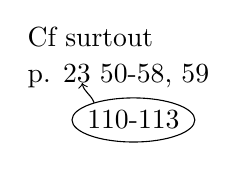
\begin{tikzpicture}[baseline=(n.base),x=1cm,y=1cm]
\node[anchor=west,inner sep=0pt] (n) at (0,0) {Cf surtout};
\node[anchor=west,inner sep=0pt] at (0,-0.5) {p. 23 \unsure{50}-\unsure{58}, 59};
\node[inner sep=1pt] (r) at (1.35,-1.05) {110-113};
\draw (1.35,-1.05) ellipse (0.78 and 0.28);
\draw[->] (0.85,-0.83) to[out=110,in=-80] (0.70,-0.58);
\end{tikzpicture}}

\uline{23 juin}

Je récapitule les données et axiomes d'une ``algèbre des figures'', ou ``\uline{atelier}''. Il s'agit pour l'instant d'axiomes purement ``algébriques'' dominant le formalisme algébrique des figures, à l'exclusion pour le moment des propriétés topologiques (densité, connexité, acyclicité) ou \inserted{proprement} géométriques (régularité topologique, boules et sphères topologiques d'une algèbre de figures), voire les ``propriété combinatoires fines'', autour de la notion de \unsure{simplexe|simplexes|simplex}.

Parmi les axiomes, je distingue les axiomes ``sine qua non'' At~1 à At~7, qui me paraissent les plus essentielles pour fonder le sens géométrico-topologique du formalisme envisagé. Les autres axiomes seront considérés comme plus ou moins ``facultatif'' au niveau du formalisme algébrique. Ils \unsure{pourront|pourraient|pourrait} \unsure{sans|donc}, \unsure{doute|donc|dans} un rôle crucial, dès qu'il s'agira d'un travail sur pièces dans le

\scanpage{3}
\mspage{2}
contexte d'un atelier définissant une ``contrée''.

Le travail précédent a permis de dégager le point de vue le plus commode pour le formalisme algébrique. La notion fondamentale me semble bien celle de \uline{figure}, et non pas celle de ``figure élémentaire'' ou ``multistrate'', voire celle de ``lieu'' (voire, la notion de ``lieu ponctuel'' ou ``point'', dont il n'a pas encore été question\ldots). Une des raisons en est la simplicité du formalisme algébrique,
% slanted
\margin{L'autre raison, c'est que, dans le cas d'une ``application $f$'' d'une ``région'' dans une autre, l'image inverse d'une ``figure'' (\unsure{quand|quant} \unsure{on} peut donner un sens \unsure{géométrique} \unsure{à} \unsure{ce} \unsure{mot|terme}) \deleted{\unsure{sera|devient|devant}} tend à ne \unsure{pas} être \unsure{encore} une figure, mais l'image réciproque d'une multistr. est une multistr.}%
 où il est agréable de pouvoir manipuler les lieux et multistrates comme étant des figures particulières. Quand une figure \inserted{$F$} est interprétée \inserted{(par l'ens de ses ``strates'')} comme partie de l'ens $\unsure{M|\mathcal M}$ \inserted{(ordonné par $\leq$)} des multistrates, nous allons écrire $\widetilde F$ (et non $F$) pour cette partie. Quand elle est interprétée comme une figure \inserted{ensembliste} dans $M$, nous l'écrivons $\mathrm{Mulomb}(F)$ (``grande multiombre''), son support est $\mathrm{Omb}(F)$ (la ``grande ombre'' de $F$) -- cette dernière, contrairement à $\widetilde F$ et à $\mathrm{Mulomb}(F)$, ne permet pratiquement jamais de réconstituer $F$, \deleted{\unsure{il|le}} mais moralement, son ``support'' seulement

\scanpage{4}
\mspage{3}
(et \unsure{je|y} suis resté muet sur ce support dans la mouture précédente GF $\underline{\overline{\mathrm{VI}}}$). Quand on interprète $F$ comme figure ensembliste dans l'\unsure{ens.|un.} des lieux $\unsure{L|\mathcal L}$ \deleted{\unsure{ou|de|ce}} (pratiquement \unsure{cela|cel} signifie qu'on a un atelier ensembliste), on l'écrira $\mathrm{mulomb}(F)$ (petite multiombre), son support sera $\mathrm{omb}(F)$.

\uline{Données} \uline{\unsure{pre|pré}\deleted{\unsure{l|li}}mières} :
\[
\left\{\begin{aligned}
&\unsure{\mathscr F|\mathcal F} &&\text{ensemble de figures}\\
&\leq &&\text{\unsure{rellation|relation} d'\uline{inclusion} \unsure{de|des} figures}\\
& &&F\leq G\ \overset{\text{\unsure{déf|def}}}{\Longleftrightarrow}\ F\ \text{sous figure de }G\\
&\ll &&\text{relation de raffinement}\\
& && F\ll G\ \overset{\text{def}}{\Longleftrightarrow}\ F\ \text{raffine }G
\end{aligned}\right.
\]
avec
\[
F\leq G\ \Longrightarrow\ F\ll G\tag*{\makebox[0pt][r]{\makebox[\displaywidth][l]{\uline{At} 0}}}
\]
% slanted
\margin{NB. Ce sera aussi contenu dans \uline{At}~4 plus bas}
-- axiome si évident que je ne l'avais pas inclus dans les axiomes numérotés.

\diagram{\(\begin{array}{@{}clp{.53\linewidth}@{}}
\text{\textcircled{\scriptsize a}} & F\vee G\ \text{ou }F\cup G &
\uline{figure} ``\uline{engendrée}'' ou ``\uline{réunion}'' ou ``\uline{somme}'' : c'est le sup au sens de $\leq$ (quand il existe\unsure{)|\}} -- auquel cas c'est aussi un sup pour $\ll$\\
\end{array}\)}
\margin{\deleted{\unsure{Question}}\inserted{NB.} : Si $(F,G)$ ont un sup pour $\ll$ (c'est tjrs le cas dans le cas ensembliste $\mathrm{Fig}(L)$), ce n'est pas néc. un sup pour $\leq$}
\margin{\uline{NB} $\widetilde{F\cap G}=\widetilde F\cap\widetilde G$}
\diagram{\(\begin{array}{@{}clp{.53\linewidth}@{}}
\text{\textcircled{\scriptsize b}} & \begin{aligned}&F\wedge G\ \text{ou } F\cap G\\&\quad(=\mathrm{Inf}^{\leq}(F,\unsure{c|G}))\end{aligned}
& figure \uline{intersection}\inserted{\tikz[x=1em,y=1em]{\draw (0,0) .. controls (-.3,.7) and (-.15,1.1) .. (.4,1.2)--(4.7,1.35)--(4.75,1.6);}\enspace ou Inf pour $\leq$} -- existe toujours \unsure{(|et (}$\overline{\mathrm m}$ pour familles infinie (non vide)) ; quand en $=$ temps $F\vee C$ existe, alors c'est aussi le Inf pour $\ll$.\\
\end{array}\)}
\margin{\uline{NB} \unsure{Exist|Existe} dans le cas ensembliste $\mathrm{Fig}(L)$ et dans le cas \unsure{mechisé|méchisé|métrisé}}
\diagram{\(\begin{array}{@{}clp{.53\linewidth}@{}}
\text{\textcircled{\scriptsize\unsure{c}}} & F\mathbin{\ldotp}G\quad (=\mathrm{Inf}^{\ll}(F,c)) &
figure ``\uline{intersection} \uline{fine} (quand elle existe) : Inf pour $\ll$.\\
&\deleted{\unsure{G|CG}}&\\
\text{\textcircled{\scriptsize\unsure{d}}} & \varnothing_{\mathscr F} &
figure vide : plus petit \unsure{élément|élémt} de $\mathscr F$ (pour $\leq$ \uline{et} pour $\ll$)\\
\end{array}\)}

\scanpage{5}
\mspage{\deleted{\unsure{3}}4}
\tikz[baseline=-.4ex,x=.75em,y=.75em]{\draw (.5,.5) circle (.48);\draw (.18,.48)--(.82,.48) (.4,.2)--(.65,.8) (.32,.76)--(.72,.23);} $M={}$ ensemble des \unsure{``}\uline{figures} $\subset\mathscr F$ \uline{élémentaires}'' ou \uline{multistrates}

\margin{\tikz[x=.6em,y=.6em]{\draw (0,1.7)--(0,2.85) .. controls (0,3.06) and (.19,3.12) .. (.50,3.12)--(2.55,3.18) .. controls (2.80,3.19) and (2.85,3.62) .. (2.88,3.9); \draw (0,1.7)--(1.20,1.72)--(2.88,1.53)--(3.02,0);}\enspace\uline{strates} d'une figure : les $X\in M$ tels que $X\leq F$\\ \uline{déployement} de $F$ : ens. de ses \uline{strates}\\ $\widetilde F=\{X\in M\mid X\leq F\}$\\ On écrit $X\triangleleft F$ ($X$ \uline{incident} à $F$) pour $X\in M$ et $X\leq F$}
\margin{formé des objets de $(\mathscr F,\leq)$ strictement irréductibles. Muni des relations $\underset{M}{\leq}$, $\underset{M}{\ll}$ induites par \deleted{\unsure{$\mathscr F$}} $\leq$ et $\ll$ dans $\mathscr F$}

\tikz[baseline=-.4ex,x=.75em,y=.75em]{\draw (.5,.5) ellipse (.43 and .55);\draw (.3,.15)--(.3,.8) (.2,.5)--(.8,.5) (.3,.66)--(.58,.9) (.3,.45)--(.62,.18);} $L\subset M$, ens. des \deleted{\uline{\unsure{éléments|points}}} \inserted{``lieux''} \deleted{\unsure{minimaux}}
\inserted{\tikz[x=.7em,y=.7em]{\draw (0,1.27)--(1.72,1.22) .. controls (2.06,1.22) and (2.42,1.02) .. (2.75,.85)--(4.67,.04)..controls(4.87,.17)and(5.17,.06)..(5.43,.08); \draw (2.57,.93)..controls(2.80,.54)and(4.13,.21)..(4.67,.04);}\enspace éléments minimaux de $\mathscr F\setminus\{\varnothing_{\mathscr F}\}$ pour $\ll$}

\uline{Axiomes}

I) Axiomes ``sine qua non''. Les premiers trois \inserted{At~1 - At~3} ne concernent que $(\mathscr F,\leq)$, les quatre suivants At~4 - At~7 \deleted{\unsure{At 1|At 4}} \deleted{\unsure{et|4}} et les relations entre $\leq$ et $\ll$

% slanted
\margin{Axiomes des \uline{sommes majorées de figures}}
\uline{At 1}\quad $\mathscr F\neq\varnothing$ et stable par $\underset{I}{\mathrm{Sup}}$ majorés ($I$ quelconque)

% slanted
\margin{Axiome des strates équivaut à :\\ Si $F,C\in\mathscr F$, alors\\ $F\leq G\Longleftrightarrow\forall X\in\widetilde F,\ \exists Y\in\widetilde G$ avec $X\leq Y$\\ Critère d'\uline{inclusion de figures par strates}}
\uline{At 2}\quad Toute figure \deleted{\unsure{d}}est le sup de ses strates :
\[
 F=\underset{X\in\widetilde F}{\mathrm{Sup}}\,X\qquad\text{où}\qquad
 \widetilde F=\{X\in M\mid X\leq F\}
\]

\uline{Scholie}\qquad \uline{At}~1 et \uline{At}~2 signifient que $\mathscr F$ s'interprète, via $F\mathrel{\tikz[baseline=-.45ex,x=.7em,y=.45em]{\draw (0,-.44)--(0,.44) (0,0)--(1.2,0) (1.2,-.44)--(1.2,.44);}}\widetilde F$, comme une partie \inserted{$\widetilde{\mathscr F}$} de $\mathscr F(M)$, $M$ ens ordonné (pour $\leq$), avec les conditions :

a) les $\Phi\in\widetilde{\mathscr F}$ sont fermés

b) Si $\Phi\in\widetilde{\mathscr F}$, toute partie fermée de $\Phi$ est $\in\widetilde{\mathscr F}$

c) $\deleted{\widetilde{\mathscr F}\neq\varnothing\quad(\Longleftrightarrow\varnothing\in\widetilde{\mathscr F})}$ (\deleted{\unsure{et}} $\displaystyle\bigcup_{\Phi\unsure{\in|+}\widetilde{\mathscr F}}\Phi=M$, et $\widetilde{\mathscr F}\neq\varnothing$
% slanted
\margin{$\widetilde{\mathscr F}\neq\varnothing$ automatique si $M\neq\varnothing$ et dans tous les cas, \unsure{équivaut} à $\varnothing\in\widetilde{\mathscr F}$}

ou, indépendamment d'une relation d'ordre sur $M$, un ens de parties satisfaisant
\diagram{\begin{tikzcd}[ampersand replacement=\&,column sep=0pt,row sep=2ex]
{} \& |[align=left,text width=.83\linewidth]| \text{b$'$)}\quad \forall x\in M,\ \text{l'ens } \widetilde{\mathscr F}^{x}=\{\deleted{\unsure{F|A}}\Phi\in\overline{\mathscr F}\mid x\in\Phi\}\ \text{a un} \\
{} \& |[align=left,text width=.83\linewidth]| \text{plus petit élément }\deleted{F}\ \text{(noté }\widetilde X\text{)}\\
{}\arrow[uu,bend left=35] \& |[align=left,text width=.83\linewidth]| \text{a$'$)}\quad\deleted{\unsure{\forall|F|\forall F}}\ \text{Dans }(\widetilde{\mathscr F},\subset),\ \text{toutes famille}\\
{} \& |[align=left,text width=.83\linewidth]| \text{majorée a un Sup, \uline{et} }\widetilde{\mathscr F}\neq\varnothing\\
{} \& |[align=left,text width=.83\linewidth]| (\Longleftrightarrow\varnothing\in\widetilde{\mathscr F})
\end{tikzcd}}

Relation
\[
\begin{aligned}
F\mathrel{\tikz[baseline=-.4ex,x=.65em,y=.65em]{\draw (0,1.1)--(1,.5)--(0,-.1) (1,1.1)--(0,.5)--(1,-.1);}}G
&\overset{\text{\unsure{dfn|défn|defn}}}{\Longleftrightarrow}
 F\vee C\ \text{existe i.e. }\{F,C\}\ \text{majoré dans }(\mathscr F,\leq)\\
&\text{\uline{figures} \uline{compatibles}}
\end{aligned}
\]
cette relation induit $X\mathrel{\tikz[baseline=-.4ex,x=.65em,y=.65em]{\draw (0,1.1)--(1,.5)--(0,-.1) (1,1.1)--(0,.5)--(1,-.1);}}Y$ dans $M$. Dans le cas où les figures sont de t.f., alors $(\mathscr F,\leq)$ \deleted{\unsure{est}} \inserted{\tikz[x=1em,y=1em]{\draw (8,1.2) .. controls (8,1) and (8,1) .. (7.7,1)--(.6,1) .. controls (.2,1) and (.2,.3) .. (0,.3);\draw (.45,.6)--(0,.3)--(.55,.28);\draw (.3,.7)--(0,.3)--(.45,.2);}\enspace avec At~1, At~2, At~3} se reconstitue par
\[
(M,\leq,\mathrel{\tikz[baseline=-.4ex,x=.65em,y=.65em]{\draw (0,1.1)--(1,.5)--(0,-.1) (1,1.1)--(0,.5)--(1,-.1);}}),\quad\text{où }\mathrel{\tikz[baseline=-.4ex,x=.65em,y=.65em]{\draw (0,1.1)--(1,.5)--(0,-.1) (1,1.1)--(0,.5)--(1,-.1);}}\text{ satisfait}
\]
\[
\left\{\begin{aligned}
&X\ \mathrel{\tikz[baseline=-.4ex,x=.65em,y=.65em]{\draw (0,1.1)--(1,.5)--(0,-.1) (1,1.1)--(0,.5)--(1,-.1);}}\ \text{réflexive symétrique}\\
&X\mathrel{\tikz[baseline=-.4ex,x=.65em,y=.65em]{\draw (0,1.1)--(1,.5)--(0,-.1) (1,1.1)--(0,.5)--(1,-.1);}}Y,\ X'\leq X,\ Y'\leq Y\ \Longrightarrow\ X'\mathrel{\tikz[baseline=-.4ex,x=.65em,y=.65em]{\draw (0,1.1)--(1,.5)--(0,-.1) (1,1.1)--(0,.5)--(1,-.1);}}Y'
\end{aligned}\right.
\]

\scanpage{6}
\mspage{5}
Donc la donnée de $(\mathscr F,\leq)$ avec figures de t.f. équivaut : $(M,\leq\deleted{\unsure{X\leq}\mathrel{\tikz[baseline=-.4ex,x=.65em,y=.65em]{\draw (0,1.1)--(1,.5)--(0,-.1) (1,1.1)--(0,.5)--(1,-.1);}}}\text{ (ordre)},\ \mathrel{\tikz[baseline=-.4ex,x=.65em,y=.65em]{\draw (0,1.1)--(1,.5)--(0,-.1) (1,1.1)--(0,.5)--(1,-.1);}}\text{ (\unsure{rel b.|rel\textsuperscript{tion}}, réflexive sym)})$ satisfaisant

a) \deleted{$\unsure{\forall x\in M}$,} \inserted{\unsure{posant}} \deleted{$\widetilde X=\{y\in M\mid y\leq x\}$ \unsure{être}} Toute partie fermée majorée $\Phi$ de $M$ est de type fini (i.e. \deleted{\unsure{$\exists$}}réunion finie d'ens. $\widetilde X=M_{\leq\unsure{x|X}}$)
\margin{On aura alors $\widetilde{\mathscr F}={}$ ens des parties fermées de $M$, de type fini, formées \unsure{de|d'} éléments deux à deux compatibles (\unsure{pour|p. r.} $\mathrel{\tikz[baseline=-.4ex,x=.65em,y=.65em]{\draw (0,1.1)--(1,.5)--(0,-.1) (1,1.1)--(0,.5)--(1,-.1);}}$)}

\[
\text{b)}\quad X\mathrel{\tikz[baseline=-.4ex,x=.65em,y=.65em]{\draw (0,1.1)--(1,.5)--(0,-.1) (1,1.1)--(0,.5)--(1,-.1);}}Y,\ X'\leq X,\ Y'\leq Y\ \Longrightarrow\ X'\mathrel{\tikz[baseline=-.4ex,x=.65em,y=.65em]{\draw (0,1.1)--(1,.5)--(0,-.1) (1,1.1)--(0,.5)--(1,-.1);}}Y'.
\]

% slanted
\margin{Critère de \uline{compatibilité} \uline{par strates}}
\uline{At 3}\quad Soient $F,G\in\mathscr F$ tels que $\forall\deleted{\unsure{x|de}}X\in\widetilde F,\ Y\in\widetilde G$, on ait $X\mathrel{\tikz[baseline=-.4ex,x=.65em,y=.65em]{\draw (0,1.1)--(1,.5)--(0,-.1) (1,1.1)--(0,.5)--(1,-.1);}}Y$, alors $F\mathrel{\tikz[baseline=-.4ex,x=.65em,y=.65em]{\draw (0,1.1)--(1,.5)--(0,-.1) (1,1.1)--(0,.5)--(1,-.1);}}G$ (i.e. $F\vee G$ existe)

\deleted{\unsure{At}} Les axiomes suivants concernent les relations entre $\leq$ et $\ll$. 1

% slanted
\margin{Critère de \uline{raffinement} \uline{par strates}\\ [\uline{Corollaire} $F\leq G\Longrightarrow F\ll G$]}
\uline{At}~4\quad $\forall F,G\in\mathscr F,$
\[
F\ll G\ \Longleftrightarrow\ \forall X\in\widetilde F,\exists Y\in\widetilde G,\ \text{t.q. }X\ll Y
\]
Ramène la connaissance de $\ll$ dans $\mathscr F$ à celle de $\underset{M}{\ll}$

% slanted
\margin{\tikz[x=.6em,y=.6em]{\draw (0,0)..controls(.6,.45)and(1.5,.58)..(2,.35); \draw (2.03,.57)--(2.3,.57);}\enspace Axiome de \unsure{la|le} plus petite strate, ou du \uline{raffinement interne} $\nearrow$}
\uline{At} \deleted{\unsure{5}}6\quad $\deleted{\forall}X,F\in\mathscr F,\ X\triangleleft F$ (i.e $X\in\widetilde F$), soit $F^{X}=\{Y\in\widetilde F\mid X\deleted{\unsure{\leq}}\ll Y\}$\unsure{,|.} Alors $F^{x}$ a un plus petit élément.

Notation
\[
\begin{aligned}
X\overset{\circ}{\ll}Y&\ \overset{\text{\unsure{dfn|df|defn|défn|déf}}}{\Longleftrightarrow}\ X\text{ est plus petit élément de }\widetilde Y^{x}\\
&\text{i.e.}\quad X\ll Y,\quad\text{et } X\ll Y'\triangleleft Y\Longrightarrow Y'=Y\\
(\text{ou } X\in\mathrm{Omb}(Y)^{\circ}) &\\
&\qquad X\ \text{\uline{raffinement interne} de }Y
\end{aligned}
\]

% slanted
\margin{\tikz[x=.6em,y=.6em]{\draw (0,0)..controls(1,.95)and(2.2,1.65)..(3.05,1.9)..controls(3.32,1.99)and(3.55,1.81)..(3.75,1.62); \draw (1.18,2.12)..controls(1.2,1.81)and(1.43,1.43)..(1.61,1.31);}\enspace équivaut à : \inserted{Si $G,H$,} \tikz[x=.6em,y=.6em]{\draw (0,0)--(.25,1.15)..controls(.32,1.45)and(.55,1.45)..(.8,1.48)--(3.3,1.62); \draw (3.3,1.62)--(3.52,1.77)--(3.68,1.58)--(3.43,1.43)--cycle;} \deleted{\unsure{Axiome}} : sont des \unsure{sous-figures|strates} d'une figure $F$, alors $F\ll G\Longleftrightarrow F\leq G$\\ (\uline{Critère du raffinement \unsure{extrinsèq.|intrinsèq.}} de \uline{figures})}
\uline{At} \deleted{\unsure{6}}5\quad Si $X\mathrel{\tikz[baseline=-.4ex,x=.65em,y=.65em]{\draw (0,1.1)--(1,.5)--(0,-.1) (1,1.1)--(0,.5)--(1,-.1);}}Y$ $(X,Y\in M)$ alors $X\ll Y\Longrightarrow X\leq Y$

ou encore, dans un $\widetilde F$, $\leq$ et $\ll$ coïncident,

ou encore, si $F,G\in M$ et $F\mathrel{\tikz[baseline=-.4ex,x=.65em,y=.65em]{\draw (0,1.1)--(1,.5)--(0,-.1) (1,1.1)--(0,.5)--(1,-.1);}}G$, alors $F\ll G\Longleftrightarrow F\leq G$.

% slanted
\margin{\tikz[x=.6em,y=.6em]{\draw (0,0)--(5,-.25); \draw (.45,.12)--(.12,0)--(.4,-.12);}\enspace \uline{Transitivité} du raffinement interne\quad\tikz[x=.6em,y=.6em]{\draw (1.18,1.8)..controls(.04,2)and(-.02,.3)..(.55,.23)..controls(.67,.2)and(.78,.24)..(.79,.32);}}
\uline{At} \deleted{\unsure{6}}7\quad Soient $X,Y,Z\in M$, alors $X\overset{\circ}{\ll}Y\overset{\unsure{\bullet|\circ}}{\ll}Z\Longrightarrow X\overset{\circ}{\ll}Z$

Traduction en termes de $(M,\leq,\ll,\widetilde{\mathscr F})$
\[
\begin{aligned}
\text{\uline{At}}_{M}\,0&\qquad \leq\ \Longrightarrow\ \ll\\
\text{\uline{A}t}_{M}\,1&\qquad \text{Les }\Phi\in\widetilde{\mathscr F}\ \text{fermés pour }\leq\\
\text{\uline{At}}_{M}\,2&\qquad\text{Si }\Phi\in\widetilde{\mathscr F},\ \Psi\ \deleted{\text{\unsure{pa}}}\text{partie fermée de }\Phi\text{ pour }<,\ \text{alors }\Psi\in\widetilde{\mathscr F}\\
&\qquad\text{et }\widetilde{\mathscr F}\neq\phi\quad(\text{i.e. }\phi\in\widetilde{\mathscr F})\\
\text{\uline{At}}_{M}\,3&\qquad\text{Si }\Phi,\Psi\in\widetilde{\mathscr F},\ \text{telles que }\forall X\in\Phi,\forall Y\in\Psi,\ \deleted{\unsure{\{X,Y\}}}X\mathrel{\tikz[baseline=-.4ex,x=.65em,y=.65em]{\draw (0,1.1)--(1,.5)--(0,-.1) (1,1.1)--(0,.5)--(1,-.1);}}Y\ (\text{i.e.}\\
&\qquad\exists\Phi\in\widetilde{\mathscr F},\ X,Y\in\Phi),\ \text{alors }\Phi\mathrel{\tikz[baseline=-.4ex,x=.65em,y=.65em]{\draw (0,1.1)--(1,.5)--(0,-.1) (1,1.1)--(0,.5)--(1,-.1);}}\Psi\quad(\text{i.e. }\Phi\mathbin{\overset{M}{\cup}}\Psi\in\widetilde{\mathscr F}).
\end{aligned}
\]

\scanpage{7}\mspage{6}
\deleted{$\mathrm{At}_{M}\,4:\ \forall X\in M,\ \unsure{\Phi|\varphi}\in\widetilde{\mathscr F}$, \unsure{posant|posons} $\Phi^{X}=\{Y\in\Phi\mid X\ll Y\}$, $\Phi^{X}$ a un plus petit \unsure{élément}}

\margin{J'ai exprimé $\uline{\mathrm{At}}\,\deleted{\unsure{6}}5$ sans référence à $\mathscr F$ ou à $\widetilde{\mathscr F}$, mais directement en termes de $(M,\leq,\ll,\mathrel{\tikz[baseline=-.4ex,x=.65em,y=.65em]{\draw (0,1.1)--(1,.5)--(0,-.1) (1,1.1)--(0,.5)--(1,-.1);}})$ $\nearrow$}%
$\mathrm{At}_{M}\,4$ \quad a) \deleted{\unsure{Posant|Posons} $X\ll Y\ \overset{\unsure{\mathrm{defn}|\mathrm{déf}}}{\unsure{\Longleftrightarrow|\Longrightarrow}}\ \unsure{Y|X}$ \unsure{contient}} \inserted{\deleted{$\forall X,Y\in M,\ X\ll$}} \inserted{\deleted{\unsure{est|ent} \unsure{minimal|minimum}}} Si $X\ll Y$, alors il y a un \deleted{\unsure{plus petit élément}} \inserted{élément minimal} \inserted{dans $\widetilde Y^{X}=\{Z\in\widetilde Y\mid X\ll Z\}$} \deleted{\unsure{i.e.} $X\ll Y'\leq Y\Longrightarrow Y'=Y$} \inserted{(posons $X\overset{\circ}{\ll}Y$ si c'est $Y$)}

\[
\begin{aligned}
\text{b) Alors}\quad & X\overset{\circ}{\ll}Y,\quad X\overset{\circ}{\ll}Y',\quad Y\mathrel{\tikz[baseline=-.4ex,x=.65em,y=.65em]{\draw (0,1.1)--(1,.5)--(0,-.1) (1,1.1)--(0,.5)--(1,-.1);}}Y'\ \Longrightarrow\ Y=Y'\\
\mathrm{At}_{M}\,\deleted{\unsure{5}}6\quad &\text{Si }X\mathrel{\tikz[baseline=-.4ex,x=.65em,y=.65em]{\draw (0,1.1)--(1,.5)--(0,-.1) (1,1.1)--(0,.5)--(1,-.1);}}Y,\ \text{alors }\ X\ll Y\ \Longrightarrow\ X\leq Y\\
\mathrm{At}_{M}\,\deleted{\unsure{6}}5\quad &X\overset{\circ}{\ll}Y\overset{\circ}{\ll}Z\ \Longrightarrow\ X\overset{\circ}{\ll}Z
\end{aligned}
\]
\margin{\tikz[x=.6em,y=.6em]{\draw (.95,0)..controls(-.3,-.15)and(-.2,1)..(.95,1.25); \draw[->] (.2,.95)..controls(-.18,1.15)and(0,2)..(.08,2.3)--(1.45,3);}}%

D'autre part, pour des $\mathscr F$ à figures de type fini, on \unsure{laisser|laisse} tomber l'élément de structure $\unsure{\widetilde{\mathscr F}|\overline{\mathscr F}}$, \inserted{au profit de $\mathrel{\tikz[baseline=-.4ex,x=.65em,y=.65em]{\draw (0,1.1)--(1,.5)--(0,-.1) (1,1.1)--(0,.5)--(1,-.1);}}$,} et remplacer $\mathrm{At}_{M}\,1$ ; $\mathrm{At}_{M}\,3$ par (a) de la \deleted{$\mathrm{At}_{M}\,\unsure{1|0}\,(\unsure{\mathrm{tf}|\mathrm{Af}|4f})$ Toute partie fermée majorée de $M$ est de t.f.} \deleted{\unsure{At}} V. \unsure{p|p.} 5 (Toute partie fermée majorée de $M$ est de t.f.) et la condition b sur $ {\mathrel{\tikz[baseline=-.4ex,x=.65em,y=.65em]{\draw (0,1.1)--(1,.5)--(0,-.1) (1,1.1)--(0,.5)--(1,-.1);}}}^{*}$. (page 5)
% slanted
\margin{i.e. $X\mathrel{\tikz[baseline=-.4ex,x=.65em,y=.65em]{\draw (0,1.1)--(1,.5)--(0,-.1) (1,1.1)--(0,.5)--(1,-.1);}}Y$ et $X'\leq X,\ Y'\leq Y$ $\unsure{\mathrel{\tikz[x=.5em,y=.28em]{\draw (0,.08)--(1.2,.08) (0,.42)--(1.2,.42) .. controls (1.35,.42) and (1.38,.23) .. (1.28,.2);}}|\Longrightarrow}X'\mathrel{\tikz[baseline=-.4ex,x=.65em,y=.65em]{\draw (0,1.1)--(1,.5)--(0,-.1) (1,1.1)--(0,.5)--(1,-.1);}}Y'$}%

Dans le cas général, quand on \unsure{à|a} simplement $\mathrel{\tikz[baseline=-.4ex,x=.65em,y=.65em]{\draw (0,1.1)--(1,.5)--(0,-.1) (1,1.1)--(0,.5)--(1,-.1);}}$ satisfaisant cette condition b) plus les conditions $\mathrm{At}_{M}\,4,5,6$, on trouve
\[
\begin{aligned}
\widetilde{\mathscr F}_{\mathrm{tf}}&=\text{ensemble des parties fermées }\inserted{\Phi\ \text{de t.f.}}\ \text{de }M,\leq\\
&\deleted{\text{\unsure{formées|fermées} \unsure{t.q.}}}\ \inserted{\text{telles que :}}\quad X,Y\in\Phi\Longrightarrow X\mathrel{\tikz[baseline=-.4ex,x=.65em,y=.65em]{\draw (0,1.1)--(1,.5)--(0,-.1) (1,1.1)--(0,.5)--(1,-.1);}}Y.
\end{aligned}
\]

Pour avoir $\widetilde{\mathscr F}$, il faut cependant un choix de structure en plus : se donner certains antifiltres infinis dans l'ens ordonné $\widetilde{\mathscr F}_{\mathrm{tf}}$ précédent\ldots

On peut aussi interpréter $\mathscr F$ en termes de
\[
\begin{aligned}
\mathscr F^{*}&=\{\mathrm{Mulomb}(F)\mid F\in\mathscr F\}\subset\mathrm{Fig}(M)\\
\deleted{\text{où}}\quad\mathrm{Mulomb}(F)&=\{\deleted{\unsure{X|\Phi}}\ \mathrm{Omb}(\unsure{x|X})\mid X\in\widetilde F\}\\
\mathrm{Omb}\,X&=\{Y\in M\mid Y\ll X\}=M_{\ll \unsure{x|X}}.
\end{aligned}
\]
(cf Scholie GF p. 28, et axiomes, ou mieux à la \uline{page 32}), comme sous-atelier (pas néc. \unsure{spacieux|spécieux}) de $\mathrm{Fig}(M)$.

% Root adjudication after blind second reading.
\scanpage{8}\mspage{7}
Je voudrais maintenant faire passer les axiomes de disjonction-compatibilité avant ceux sur les lieux, pour ne pas \inserted{avoir l'air de} les en faire dépendre. Les axiomes sont ``facultatif\unsure{s}'' pour un atelier, et il y aura pas mal des' implications mutuelles avec les axiomes sur les lieux.

Une notion essentielle ici est celle de ``$F$ et $\unsure{G|C}$ \uline{disjoints}''
\[
 F\parallel\unsure{G|C}\ \overset{\unsure{\mathrm{dfn}|\mathrm{defn}|\mathrm{def}}}{\Longleftrightarrow}\ F\mathrel{\tikz[baseline=-.4ex,x=.65em,y=.65em]{\draw (0,1.1)--(1,.5)--(0,-.1) (1,1.1)--(0,.5)--(1,-.1);}}G\quad\text{et}\quad F\cap C=\varnothing_{\mathscr F}
\]
notion qui ne dépend que de $\leq$. On a d'ailleurs
\[
 F\parallel G\ \Longleftrightarrow\ \forall X\in\widetilde F,\ Y\in\widetilde G,\quad X\parallel Y
\]
donc interprétation en \unsure{termes|terme} de $X\parallel Y$ dans $M$, qui y signifie
\[
\begin{aligned}
X\mathrel{\underset{M}{\parallel}}Y\ \Longleftrightarrow\
 X\mathrel{\underset{M}{\mathrel{\tikz[baseline=-.4ex,x=.65em,y=.65em]{\draw (0,1.1)--(1,.5)--(0,-.1) (1,1.1)--(0,.5)--(1,-.1);}}}}Y\quad &\text{et}\quad\{X,Y\}\ \text{n'est \uline{pas}}\\
&\text{minoré dans } M,\leq\\
&\text{i.e. }\nexists Z\ \text{avec }Z\leq X,Z\leq Y
\end{aligned}
\]

(\uline{NB} Il résul\deleted{\unsure{tera}}\inserted{te} des axiomes \inserted{précédents} que ça implique que $\nexists Z$ avec $Z\ll X,Z\ll Y$, \deleted{\unsure{i.e.} \unsure{c'est un} $\unsure{\exists|]}$} et \deleted{\unsure{la}} réciproque résultera \unsure{d'axiome|d'axiomes} ci-dessous\ldots)

% slanted
\margin{\unsure{Un atelier sera dit \uline{spacieux} s'il satisfait cette condition. Contre-ex. : les ateliers simpliciaux\ldots|\deleted{Un atelier sera dit \uline{spacieux} s'il satisfait cette condition. Contre-ex. : les ateliers simpliciaux\ldots}}}%
\deleted{\uline{At DC} 1 \quad (\uline{Axiome des ateliers spacieux}) \unsure{Soient} $X,Y\in M$, \inserted{soit} \deleted{\unsure{et}} $K=X\cap Y=\underset{Z\in\widetilde X\cap\widetilde Y}{\mathrm{Sup}}\,Z$. \deleted{\unsure{Il}} Supposons que \inserted{pour $X',Y'\in M$}}
\[
\deleted{\deleted{\unsure{\forall}}\ X'\ll X,\ X'\parallel K,\ Y'\ll Y,\ Y'\parallel K\ \Longrightarrow\ X'\parallel Y'.}
\]
\deleted{Alors [NB et alors seulement\ldots\ \inserted{cf Cor}] $X\mathrel{\tikz[baseline=-.4ex,x=.65em,y=.65em]{\draw (0,1.1)--(1,.5)--(0,-.1) (1,1.1)--(0,.5)--(1,-.1);}}Y$.}

\deleted{\uline{Cor} Soient $F,G\in\mathscr F$, $K=F\cap\unsure{C|G}=\underset{Z\in\deleted{\unsure{\widetilde X|X}}F\cap\deleted{\unsure{\widetilde Y|Y}}\unsure{\widetilde G|\widetilde C}}{\mathrm{Sup}}\,Z$.}
\[
\begin{aligned}
&\deleted{\text{Alors } F\mathrel{\tikz[baseline=-.4ex,x=.65em,y=.65em]{\draw (0,1.1)--(1,.5)--(0,-.1) (1,1.1)--(0,.5)--(1,-.1);}}C\quad \text{\tikz[baseline=(s.base)]{\node[inner sep=1pt] (s) {ses};\draw (s.center) ++(30:1.05em and .72em) arc[start angle=30,end angle=-295,x radius=1.05em,y radius=.72em];}}\quad \forall X,\deleted{\unsure{\varphi|y}}\unsure{Y|y}\in M}\\
&\deleted{X\ll F,\ Y\ll C,\ X\parallel K,\ Y\parallel K\ \Longrightarrow\ X\parallel Y}
\end{aligned}
\]

\scanpage{9}\mspage{8}
J'explicite, à cause de son importance, la propriété suivante, bien qu'elle sera conséquence de diverses façons d'autres

\deleted{\uline{At} DC 1 : Soient $X,Y\in M$ avec $\unsure{X|X'}\deleted{\unsure{\parallel}}\mathrel{\tikz[baseline=-.4ex,x=.65em,y=.65em]{\draw (0,1.1)--(1,.5)--(0,-.1) (1,1.1)--(0,.5)--(1,-.1);}}Y\unsure{\text{\S}|?|.}$}
\deleted{\deleted{\unsure{Alors|At}} \inserted{Soient} $X'\ll X$, \deleted{$Y'\ll Y\Longrightarrow X'\parallel\unsure{Y'|Y}$} \inserted{avec $X'\parallel X\cap Y=L$, (i.e. $X'\parallel Z$ pour $Z\leq X,Y$} $Y'\ll Y$ avec $Y'\parallel L$. Alors $X'\parallel Y'$}

% slanted
\margin{\uline{NB} La chose importante est $X'\mathrel{\tikz[baseline=-.4ex,x=.65em,y=.65em]{\draw (0,1.1)--(1,.5)--(0,-.1) (1,1.1)--(0,.5)--(1,-.1);}}Y'$, alors $X'\cap Y'=\unsure{\phi|\varnothing}$ immédiat. Car $Z\deleted{\ll}\leq X',\,Z\leq Y'$ $\Longrightarrow Z\ll X,\,Z\ll\unsure{Y'|Y}$ d'où $Z\ll X\cap Y=L$, or $Z\leq X'\parallel L\underset{\mathrm{At}}{\Longrightarrow}Z\parallel L$, or $Z\ll L$ et $Z\parallel L$ c'est \deleted{\unsure{impossible}} (\unsure{comme|d'où} $Z\mathrel{\tikz[baseline=-.4ex,x=.65em,y=.65em]{\draw (0,1.1)--(1,.5)--(0,-.1) (1,1.1)--(0,.5)--(1,-.1);}}L$) $\Longrightarrow Z^{+}\leq L$ \unsure{\deleted{absurde}|absurde} car \uline{$Z\cap L=\phi$ !}}%
% Connected thin upper, right-side and lower-oblique strokes crossing/bordering the NB note.
\margin{\tikz[x=.45em,y=.45em]{\draw (0,0)--(4,0);\draw (3.4,.2)--(3.6,-10);\draw (1.4,-6.4)--(3.9,-8.7);}}

\deleted{\uline{Cor} 1 Soient $F,C\in\mathscr F$ avec $F\parallel C$. Alors $F\ll F$, $C'\ll G\Longrightarrow F'\parallel G'$.}
\deleted{\uline{Cor. 2} Soient $F,G\in\mathscr F$, $F\mathrel{\tikz[baseline=-.4ex,x=.65em,y=.65em]{\draw (0,1.1)--(1,.5)--(0,-.1) (1,1.1)--(0,.5)--(1,-.1);}}G$ \deleted{\unsure{avec} $\unsure{L=\underset{Z\in\widetilde F\cap\widetilde G}{\mathrm{Sup}}\,Z}$} \inserted{$L=F\cap G$}, $F'\ll F,C'\ll G$. Supposons $F'\parallel L,\ C'\parallel L$, alors $F'\parallel G'$.}

\deleted{\uline{At DC} 2 \quad (Axiome des ateliers \unsure{spacieux|spécieux}) \deleted{\unsure{Soit|Soient}} $X,Y\in M$, $\deleted{\unsure{L}}K=X\cap Y=\underset{Z\in\widetilde X\cap\widetilde Y}{\mathrm{Sup}}\,Z$. Supposons que pour tt $X',Y'$, avec $X'\ll X,\underset{\tikz[x=1em,y=.35em,baseline=0pt]{\draw (0,0) .. controls (1,-.05) and (2,-.05) .. (3.4,.40);\draw (1.66,.16)--(1.85,.01)--(1.67,-.13);}}{Y'\ll Y,\ X'\parallel K},Y'\parallel K$, on ait $X'\parallel Y'$. Alors}

% Editing stroke beneath the preceding cancelled draft, with left oblique and rising right end.
\noindent\tikz[x=1em,y=1em]{\draw (0,.03) .. controls (2,.15) and (4,.18) .. (6,.12) .. controls (8,-.04) and (10,-.10) .. (11.1,-.08) .. controls (11.45,.55) and (11.55,.95) .. (12.2,1.18);\draw (-.18,-.03)--(.95,1.32);}

On voudra la

\uline{Propriété 1} Soient $F,G\in\mathscr F$, $F\mathrel{\tikz[baseline=-.4ex,x=.65em,y=.65em]{\draw (0,1.1)--(1,.5)--(0,-.1) (1,1.1)--(0,.5)--(1,-.1);}}G$, $L=F\cap G$. Soient $F'\ll F,\ G'\ll G$. Alors
\[
\begin{aligned}
 & F'\mathrel{\tikz[baseline=-.4ex,x=.65em,y=.65em]{\draw (0,1.1)--(1,.5)--(0,-.1) (1,1.1)--(0,.5)--(1,-.1);}}G'\\
\Longleftrightarrow\quad & F'_{L}\mathrel{\tikz[baseline=-.4ex,x=.65em,y=.65em]{\draw (0,1.1)--(1,.5)--(0,-.1) (1,1.1)--(0,.5)--(1,-.1);}}G'_{L}
\end{aligned}
\]

cf \deleted{\unsure{p.}} GF $\underline{\overline{\mathrm{VI}}}$, p.~\uline{\unsure{73|13}} -- On a en tous cas tjrs $\unsure{\mathrel{\tikz[x=.5em,y=.28em]{\draw (0,.08)--(1.2,.08) (0,.42)--(1.2,.42) .. controls (1.35,.42) and (1.38,.23) .. (1.28,.2);}}|\Rightarrow}$
\deleted{\unsure{Montrons} qu'on a bien \unsure{en} $\Rightarrow$. En effet,}

Ceci est équivalent (si on le voit de façon générale) à l'ancien At 12, qui prend le nom

% slanted
\margin{\uline{Critère} de \uline{compatibilité} pour les raffinements de \uline{sous-figures}\quad Mais c'est faux dans le cas simplicial, ex :}%
\figure{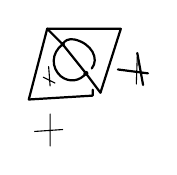
\begin{tikzpicture}[x=.035em,y=-.035em,line cap=round,line join=round]
\draw[thick] (30,10)--(106,10)--(85,76);
\draw[thick] (30,10)--(11,83)--(77,79)--(77,73);
\draw[thick] (30,10)--(46,26)--(70,56)--(85,76);
\draw[thick] (76,51) .. controls (84,41) and (76,25) .. (58,21)
 .. controls (52,20) and (48,22) .. (46,26)
 .. controls (34,35) and (34,50) .. (44,59)
 .. controls (53,66) and (64,64) .. (70,56);
\fill (46,26) circle (2.2) (70,56) circle (2.6);
\draw (26,60)--(38,66) (31.5,49)--(33,69);
\draw[thick] (103,52)--(134,56) (123,35)--(129,68);
\draw (123,39)--(122,67);
\draw (17,116)--(46,114) (33,98)--(33,131);
\end{tikzpicture}}
% slanted
\margin{Mais on aura $X'_{L}\parallel Y'_{L}\Longrightarrow X'\mathrel{\tikz[x=.55em,y=.60em,line cap=round]{\draw (0,-.12)--(0,1) (.48,-.12)--(.48,1) (-.06,.30)--(.54,.47) (-.05,.51)--(.53,.65);}}Y'$, C'est un contre-exple à l' : At $\unsure{\parallel|11}$, et a fortiori à \deleted{\unsure{ex}} At 11 (cf GF $\underline{\overline{\mathrm{VI}}}$, p. 67,68)}%

% Vertical rule bordering the axiom on its left.
\margin{\tikz[x=.5em,y=.5em]{\draw (0,0)--(0,4.25);}}
\uline{At DD} 1 Soient \inserted{ou bien} $X,Y\ \&\ X',Y'\in M$, $X\mathrel{\tikz[baseline=-.4ex,x=.65em,y=.65em]{\draw (0,1.1)--(1,.5)--(0,-.1) (1,1.1)--(0,.5)--(1,-.1);}}Y,\ X'\ll X,Y'\ll Y$. Posons $K=X\cap Y=\underset{Z\in\widetilde X\cap\widetilde Y}{\mathrm{Sup}}\,Z$. Alors $X'_{L}\mathrel{\tikz[baseline=-.4ex,x=.65em,y=.65em]{\draw (0,1.1)--(1,.5)--(0,-.1) (1,1.1)--(0,.5)--(1,-.1);}}Y'_{L}$ implique $X'\mathrel{\tikz[baseline=-.4ex,x=.65em,y=.65em]{\draw (0,1.1)--(1,.5)--(0,-.1) (1,1.1)--(0,.5)--(1,-.1);}}Y'$ \quad (NB l'inverse \deleted{\unsure{est}} tjrs vrai)

\uline{\unsure{Cor. Main|Corollaire}} 1 \quad \unsure{la|le} ``propriété'' ci dessus

\[
F\parallel G,\ F'\ll F,\ C'\ll G\ \Longrightarrow\ F'\parallel G'
\tag*{\makebox[0pt][r]{\makebox[\displaywidth][l]{\uline{\unsure{Cor. Main|Corollaire}} 2}}}
\]

Plus gén. \quad Si $F\mathrel{\tikz[baseline=-.4ex,x=.65em,y=.65em]{\draw (0,1.1)--(1,.5)--(0,-.1) (1,1.1)--(0,.5)--(1,-.1);}}G,\ F'\ll F,\ C'\ll G$, alors
\[
 F'\parallel G'\ \Longleftrightarrow\ F'_{L}\parallel G'_{L}
\]
